\documentclass[twocolumn, 11pt, letterpaper]{article}

% ── Paquetes ─────────────────────────────────────────────────
\usepackage[utf8]{inputenc}
\usepackage[T1]{fontenc}
\usepackage[spanish, es-tabla]{babel} 
\usepackage{amsmath, amssymb}
\usepackage{geometry}
\usepackage{graphicx}
\usepackage{booktabs}
\usepackage{enumitem}
\usepackage[hidelinks]{hyperref}
\usepackage{fancyhdr}
\usepackage{titlesec}
\usepackage{parskip}
\usepackage{xcolor}
\usepackage{caption}
\usepackage{float}
\usepackage{tabularx}
\usepackage{listings}
\usepackage{xcolor}


\definecolor{jsonkey}{rgb}{0,0,1}
\definecolor{jsonstring}{rgb}{0,0.5,0}

\lstset{
    basicstyle=\ttfamily\tiny, % Fuente muy pequeña para ahorrar espacio
    breaklines=true,
    showstringspaces=false,
    commentstyle=\color{gray},
    keywordstyle=\color{jsonkey},
    stringstyle=\color{jsonstring},
    frame=single,
    captionpos=b
    }

% ── Geometría ────────────────────────────────────────────────
\geometry{
  letterpaper,
  top=2.5cm,
  headheight=15pt,
  bottom=2.2cm,
  left=1.8cm, right=1.8cm,
  columnsep=0.7cm
}

% ── Formato de secciones  ─────────────────────────
\titleformat{\section}
  {\normalfont\bfseries\large}{\thesection.}{0.5em}{}
  [\vspace{-3ex}\rule{\columnwidth}{0.4pt}] % Vspace negativo para subir la línea

\titlespacing{\section}
  {0pt}{0ex }{0ex} 
  % {izq}{arriba}{distancia entre línea y texto}

\titleformat{\subsection}
  {\normalfont\bfseries\normalsize}{\thesubsection.}{0.5em}{}

% ── Encabezado y pie ─────────────────────────────────────────
\pagestyle{fancy}
\fancyhf{}
\fancyhead[L]{%
  \begin{picture}(0,0)
    \put(-13.5, -63){
\includegraphics[height=5.1cm]{logonegrousm}}
  \end{picture}
}
\fancyhead[C]{\small\textbf{ICN292} -- Sistemas de información para la gestión}
\fancyhead[R]{\small Automatización Cursor}
\fancyfoot[C]{\thepage}
\renewcommand{\headrulewidth}{0.4pt}

\begin{document}

% ── Título───────────────────────────────────
\twocolumn[{%
\vspace*{-0.5cm}
\begin{center}
  {\LARGE \textbf{\textit{Cursor} -- Conversión de Formato de texto Local}}\\[4pt]
  {\large Sistemas de información para la gestión -- ICN292}\\[6pt]
  \begin{tabular}{ll}
    \textit{Benjamín Jara}  & \textit{21.469.796-3} \\
  \end{tabular}\\[4pt]
  {\small Universidad Técnica Federico Santa María \quad $\cdot$ \quad Semestre 2026-1 $\cdot$ \quad 05 de Junio}\\[3pt]
  \rule{\textwidth}{0.6pt}\\[5pt]
\end{center}
}]

\section{Introducción}
Se presenta \textbf{Cursor} en su versión gratuita (ver \hyperref[fig:version_gratuita]{Anexo~\ref*{fig:version_gratuita}})como agente que opera a nivel local, lo cual se diferencia de las inteligencias artificiales convencionales principalmente por la capacidad de acceso a información en el ambiente local que puede acceder.


Cursor es un agente que es capaz de operar dentro de las carpetas locales del sistema, tomando como contexto el ambiente del computador para proporcionar respuestas más adecuadas, lo cual, lo hace capaz de comprender de manera más eficiente el proceso a ejecutar, o las consultas que se deseen realizar sobre el ambiente.

El programa presenta un enfoque orientado a la estructura de datos, pues su fuerte es entender la contextualización de los problemas o las consultas que uno realice, donde es capaz de generar archivos y carpetas desde 0 o bien, modificar archivos de manera directa, como puede ser un archivo de código de Python, donde puede modificar línea por línea de ser necesario.

Todo esto abre la posibilidad de automatizar procesos, que bien pueden ser locales, pero por la necesidad de herramientas más robustas, se requiere una herramienta capaz de sintetizar de mejor manera y con la finalidad de utilizar las herramientas adquiridas en proyectos anteriores, se recurre a la \textit{API key} de gemini, para que esta sea quien procese los archivos y la sintetización del código.

\section*{Proceso a automatizar}

Se busca automatizar la creación del archivo LaTeX a partir de un archivo PDF cualquiera, sea en formato digital o texto plano, debido a la complejidad del problema, la estructura base del formato en LaTeX, incluyendo la información, la creación de una estructura básica si es que corresponde junto con formalidades estándares.


\section*{Descripción Técnica}

Se detallan los Pasos esenciales de la resolución.

\section*{Archivos involucrados}

El proceso opera sobre los siguientes archivos locales:

\begin{itemize}
    \item \texttt{input/} --- carpeta de entrada donde el usuario deposita el PDF a convertir.
    \item \texttt{output/} --- carpeta de salida donde el script deposita el \texttt{.tex} generado y el \texttt{.pdf} compilado.
    \item \texttt{template.tex} --- archivo base que define el formato del documento LaTeX: dos columnas, encabezado con sigla y ramo, geometría de página y estilo de secciones de la UTFSM.
    \item \texttt{logonegrousm.png} --- logo institucional copiado automáticamente a \texttt{output/} para que \texttt{pdflatex} pueda incluirlo en la compilación.
    \item \texttt{.env} --- archivo de configuración que contiene la API key de Gemini, mantenida fuera del código por seguridad.
    \item \texttt{converter.py} --- script principal que orquesta todo el proceso.
\end{itemize}

\section*{Flujo de datos}

Al detectar un PDF en \texttt{input/}, el script lee el archivo en bytes
junto con el contenido de \texttt{template.tex} y los envía a la API de
Gemini mediante una solicitud HTTP\@. Gemini recibe el PDF completo y el
template como contexto, y genera el código LaTeX respetando exactamente
la estructura definida. El script guarda la respuesta como \texttt{.tex}
en \texttt{output/}, copia el logo si existe, y ejecuta \texttt{pdflatex}
dos veces localmente para compilar el PDF final y resolver referencias
cruzadas.
\section*{Uso del chat con contexto (\texttt{@})}

Una de las funcionalidades centrales de Cursor es la posibilidad de
referenciar archivos del proyecto directamente en el chat mediante el
operador \texttt{@}. Durante el desarrollo, se consultó al asistente
referenciando \texttt{@converter.py} para preguntar cómo manejar el caso
en que el archivo PDF recibido estuviera corrupto o vacío. Cursor leyó
el contenido real del archivo y propuso una validación previa al envío
a Gemini, verificando que el archivo tuviera un tamaño mayor a cero y
que sus primeros bytes correspondieran a la firma \texttt{\%PDF-}.
Esto permitió incorporar manejo de errores específico al contexto del
proyecto, sin necesidad de buscar soluciones genéricas externas.
\begin{figure}[H] 
    \centering
    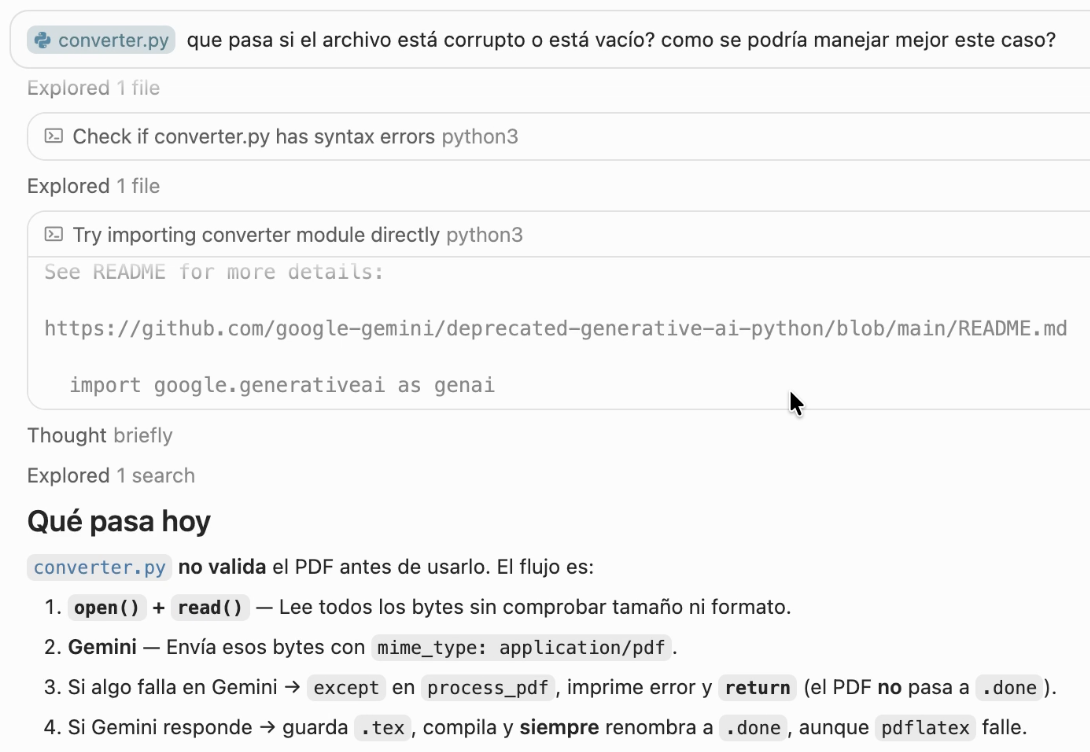
\includegraphics[width=1\linewidth]{consultasarroba.png}
    \caption{Consulta sobre archivo específico.}
    \label{fig:placeholder}
\end{figure}
\section*{Edición asistida con \texttt{Cmd+K}}

Durante el desarrollo, se seleccionó el bloque correspondiente al
\texttt{prompt} enviado a Gemini en \texttt{converter.py} y se utilizó
la edición inline mediante \texttt{Cmd+K}. Se solicitó al asistente
mejorar el prompt para que fuera más estricto con el formato de
ecuaciones matemáticas y expresiones simbólicas. Cursor generó una
versión extendida del prompt incorporando instrucciones explícitas sobre
el uso de entornos matemáticos de \LaTeX, aplicando el cambio
directamente sobre el archivo mediante un diff visual que permitió
revisar y aceptar las modificaciones línea por línea, sin salir del
editor.
\begin{figure}[H]
    \centering
    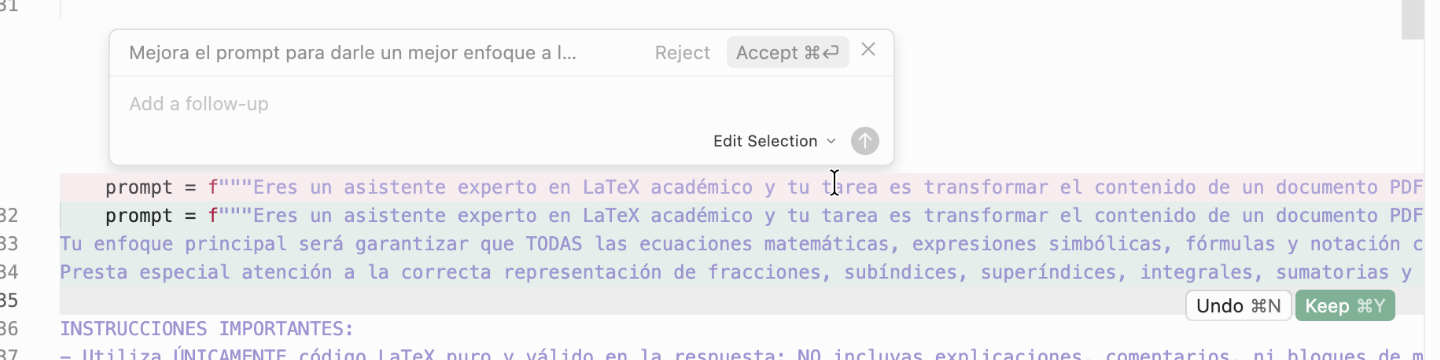
\includegraphics[width=\columnwidth]{cmdk.png}
    \caption{Edición Prompt con Cmd+k.}
    \label{fig:etiqueta}
\end{figure}

\section*{Ejecución del script}

El script se ejecuta desde la terminal integrada de Cursor mediante
el comando \texttt{python3 converter.py}. Al iniciarse, el programa
desplegó un mensaje de confirmación indicando que el monitor estaba
activo sobre la carpeta \texttt{input/}. Al depositar un PDF de prueba, el cual corresponde a un certamen con pauta del ramo Econometría, el script
detectó el archivo automáticamente, realizó la llamada a la API de
Gemini, guardó el archivo \texttt{.tex} resultante en \texttt{output/},
copió el logo institucional, ejecutó \texttt{pdflatex} en dos pasadas
y eliminó los archivos auxiliares generados por la compilación. El PDF
original quedó renombrado con extensión \texttt{.done} como señal de
que fue procesado correctamente. El resultado final en \texttt{output/}
consistió en el código fuente \texttt{.tex} y el documento \texttt{.pdf}
compilado con el formato de dos columnas y encabezado institucional de
la UTFSM\@.
\begin{figure}[H] 
    \centering
    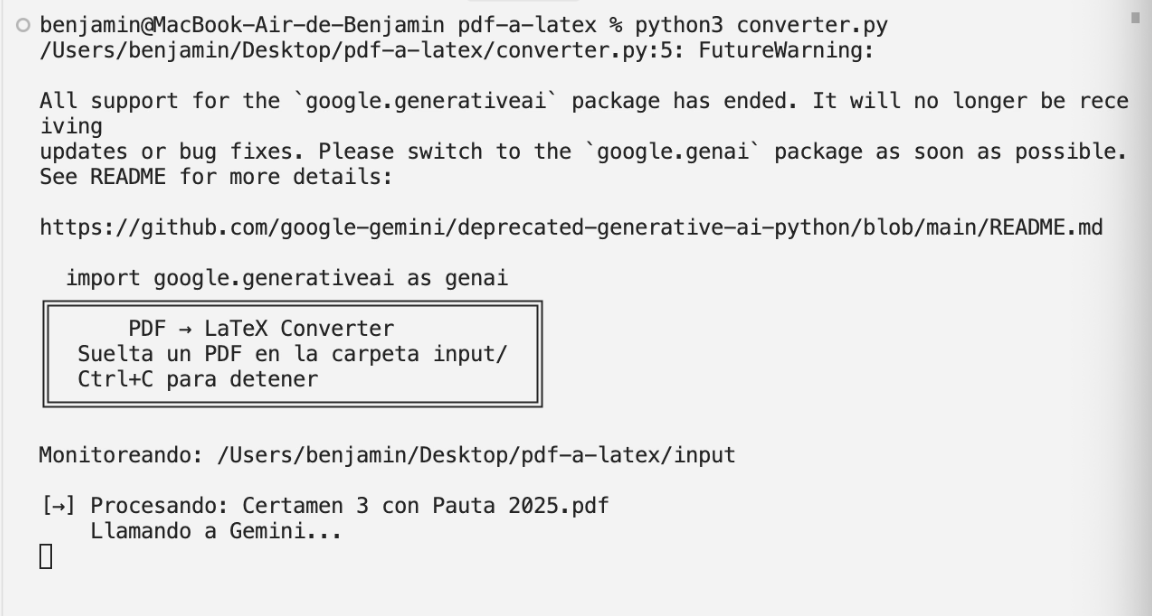
\includegraphics[width=1\linewidth]{terminal.png}
    \caption{Ejecución del script de Python mediante terminal.}
    \label{fig:placeholder}
\end{figure}

\section*{Conclusión}
Cursor es una herramienta útil para el manejo de archivos de diversa naturaleza, la capacidad de entender desde adentro la problemática tomando como contexto los archivos permite una manera de operar más eficiente, ahorrándose la necesidad de instruir a las inteligencias artificiales con los archivos cada vez que se requiera hacer una consulta.
Además, la herramienta permite la creación de archivos, que expande las posibilidades de creación de contenido útil para el día a día, como en este caso, cursor se vuelve el actor principal que monitorea el proceso completo de conversión de pdf a latex, pues como el proceso puede fallar una infinidad de veces, Cursor se vuelve el agente ideal para monitorear donde fracasa el conjunto y es capaz de arreglarlo sobre la marcha.
Se destaca y valora principalmente el manejo de datos de manera eficaz y rápida, sin la necesidad de adjuntar archivos cada vez que se quiere consultar algo nuevo o complementar información ya discutida.
Como limitación principal se destaca el uso muy limitado de la aplicación por el plan gratuito, fuera de eso, la herramienta se destaca como una opción robusta para el manejo de datos de manera local.
Es importante mencionar que el flujo  (ver \hyperref[fig:version_gratuita]{Anexo~\ref*{fig:flujo_lucid}}), depende de cursor y puede no siempre ser el mismo, pues frente a la falla, cursor toma rutas alternativas que dependen de cada problema específico.
\onecolumn
\section*{Anexo}
\setcounter{figure}{0}
\begin{figure}[H] 
    \centering
    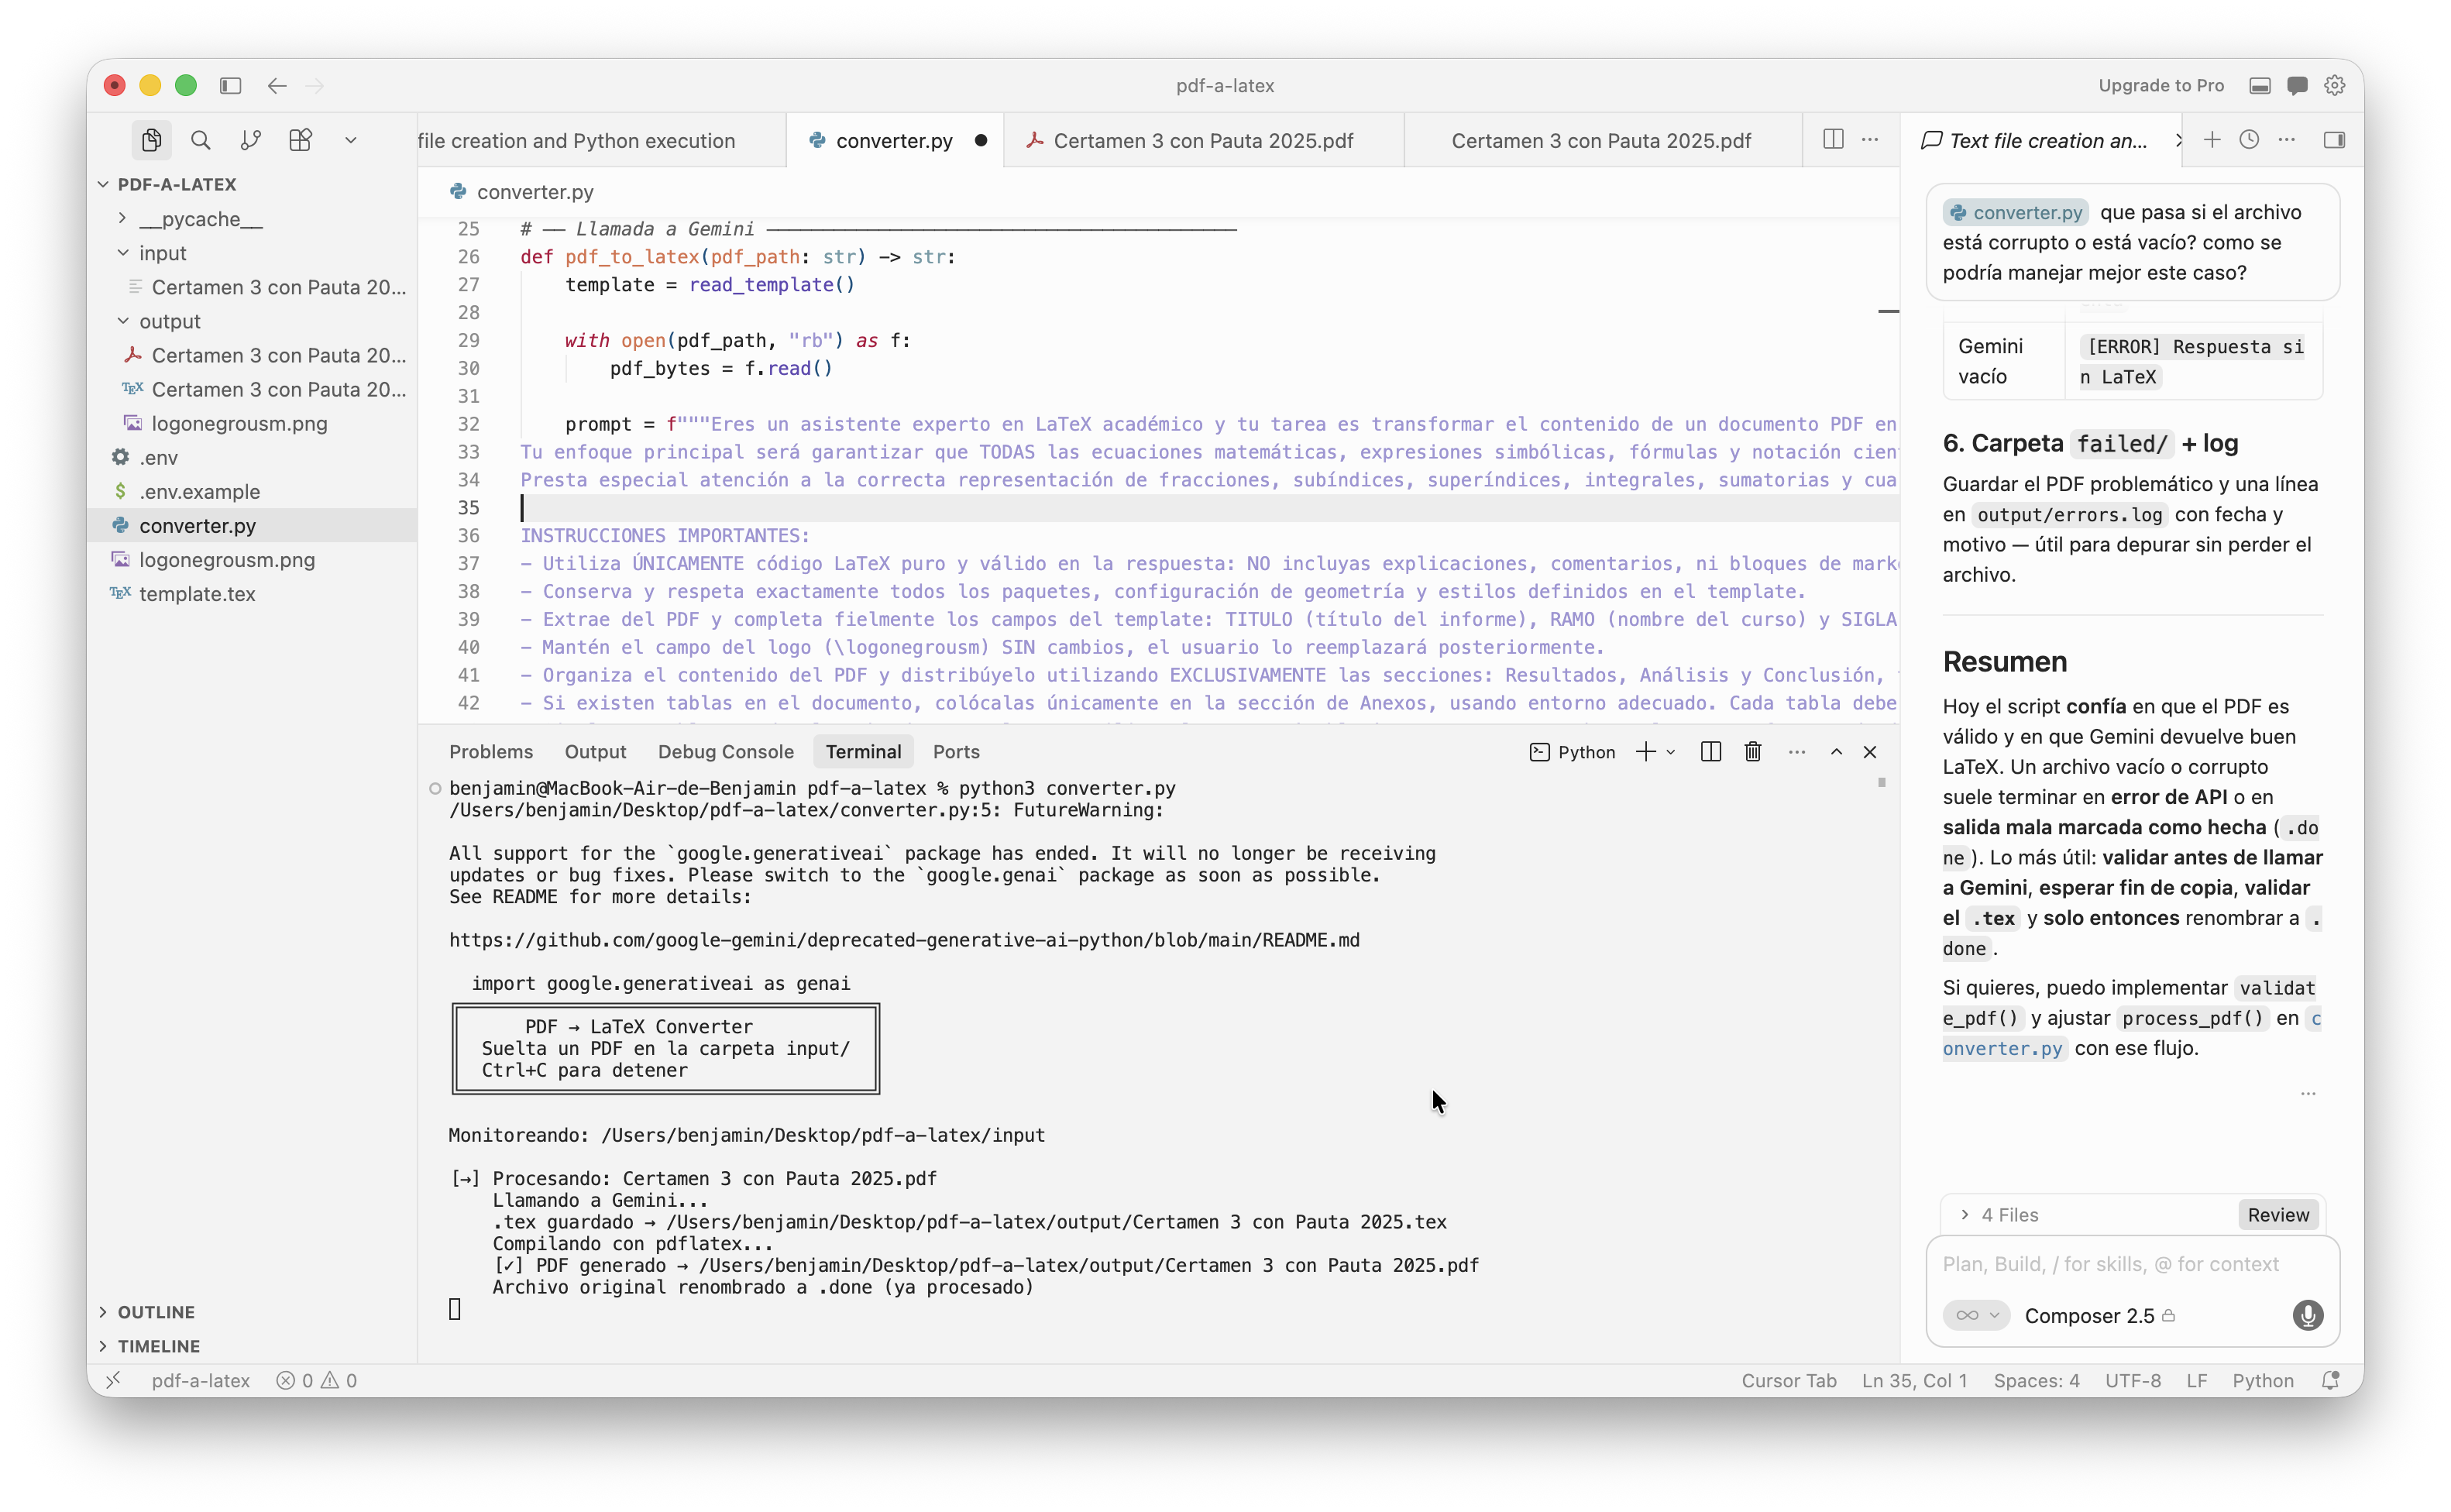
\includegraphics[width=\columnwidth]{Evidenciadeuso.png}
    \caption{Evidencia de uso de Cursor: Se puede apreciar arriba a la derecha, que, existe el botón de "Upgrade to Pro", lo cual significa que se usó la versión gratuita.}
    \label{fig:version_gratuita}
\end{figure}
\begin{figure}[H] 
    \centering
    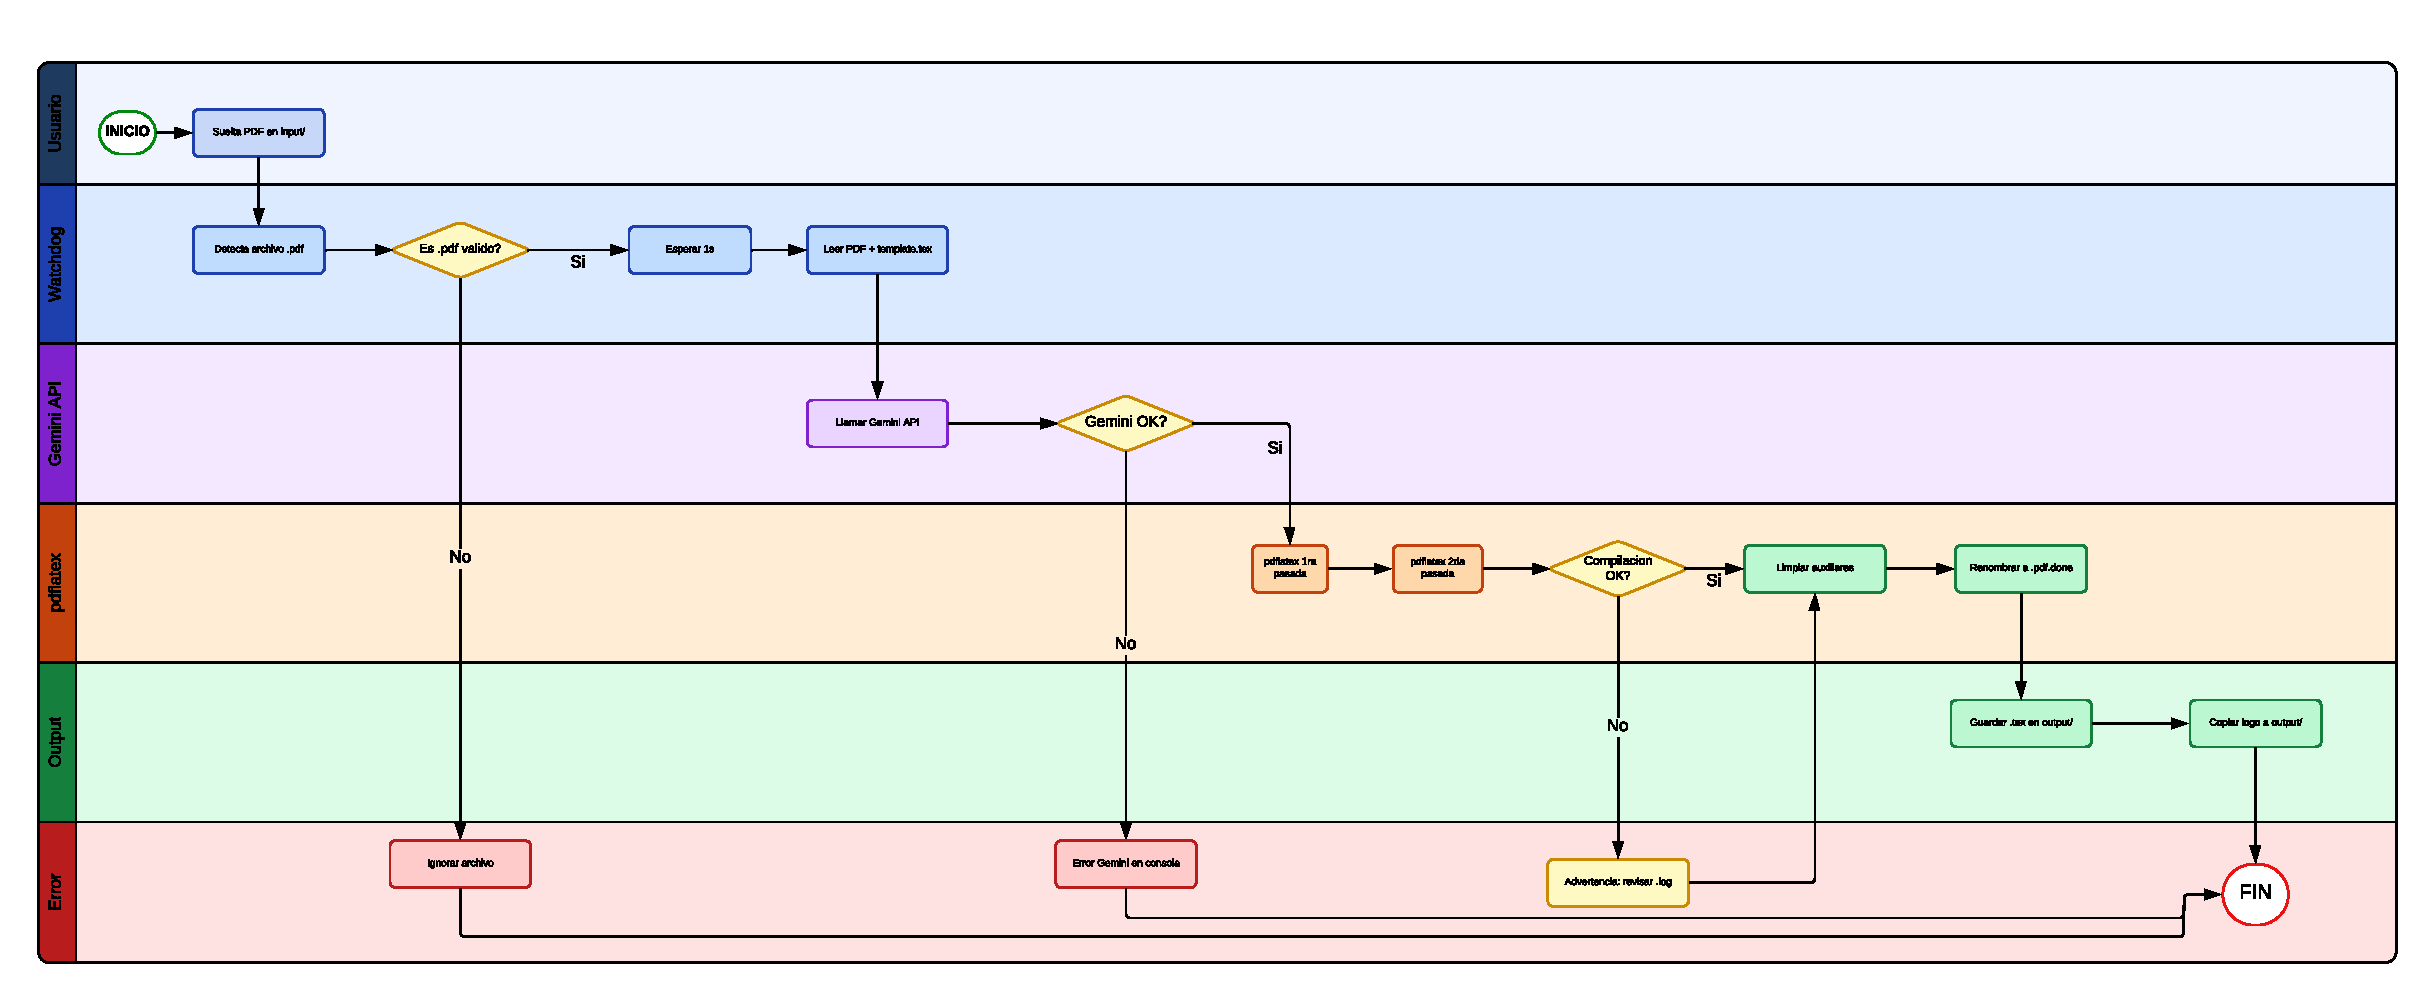
\includegraphics[width=\columnwidth]{FlujoCursor.pdf}
    \caption{Diagrama de procesos diseñado en Lucidchart.}
    \label{fig:flujo_lucid}
\end{figure}


\end{document}
\begin{figure}
    \centering
    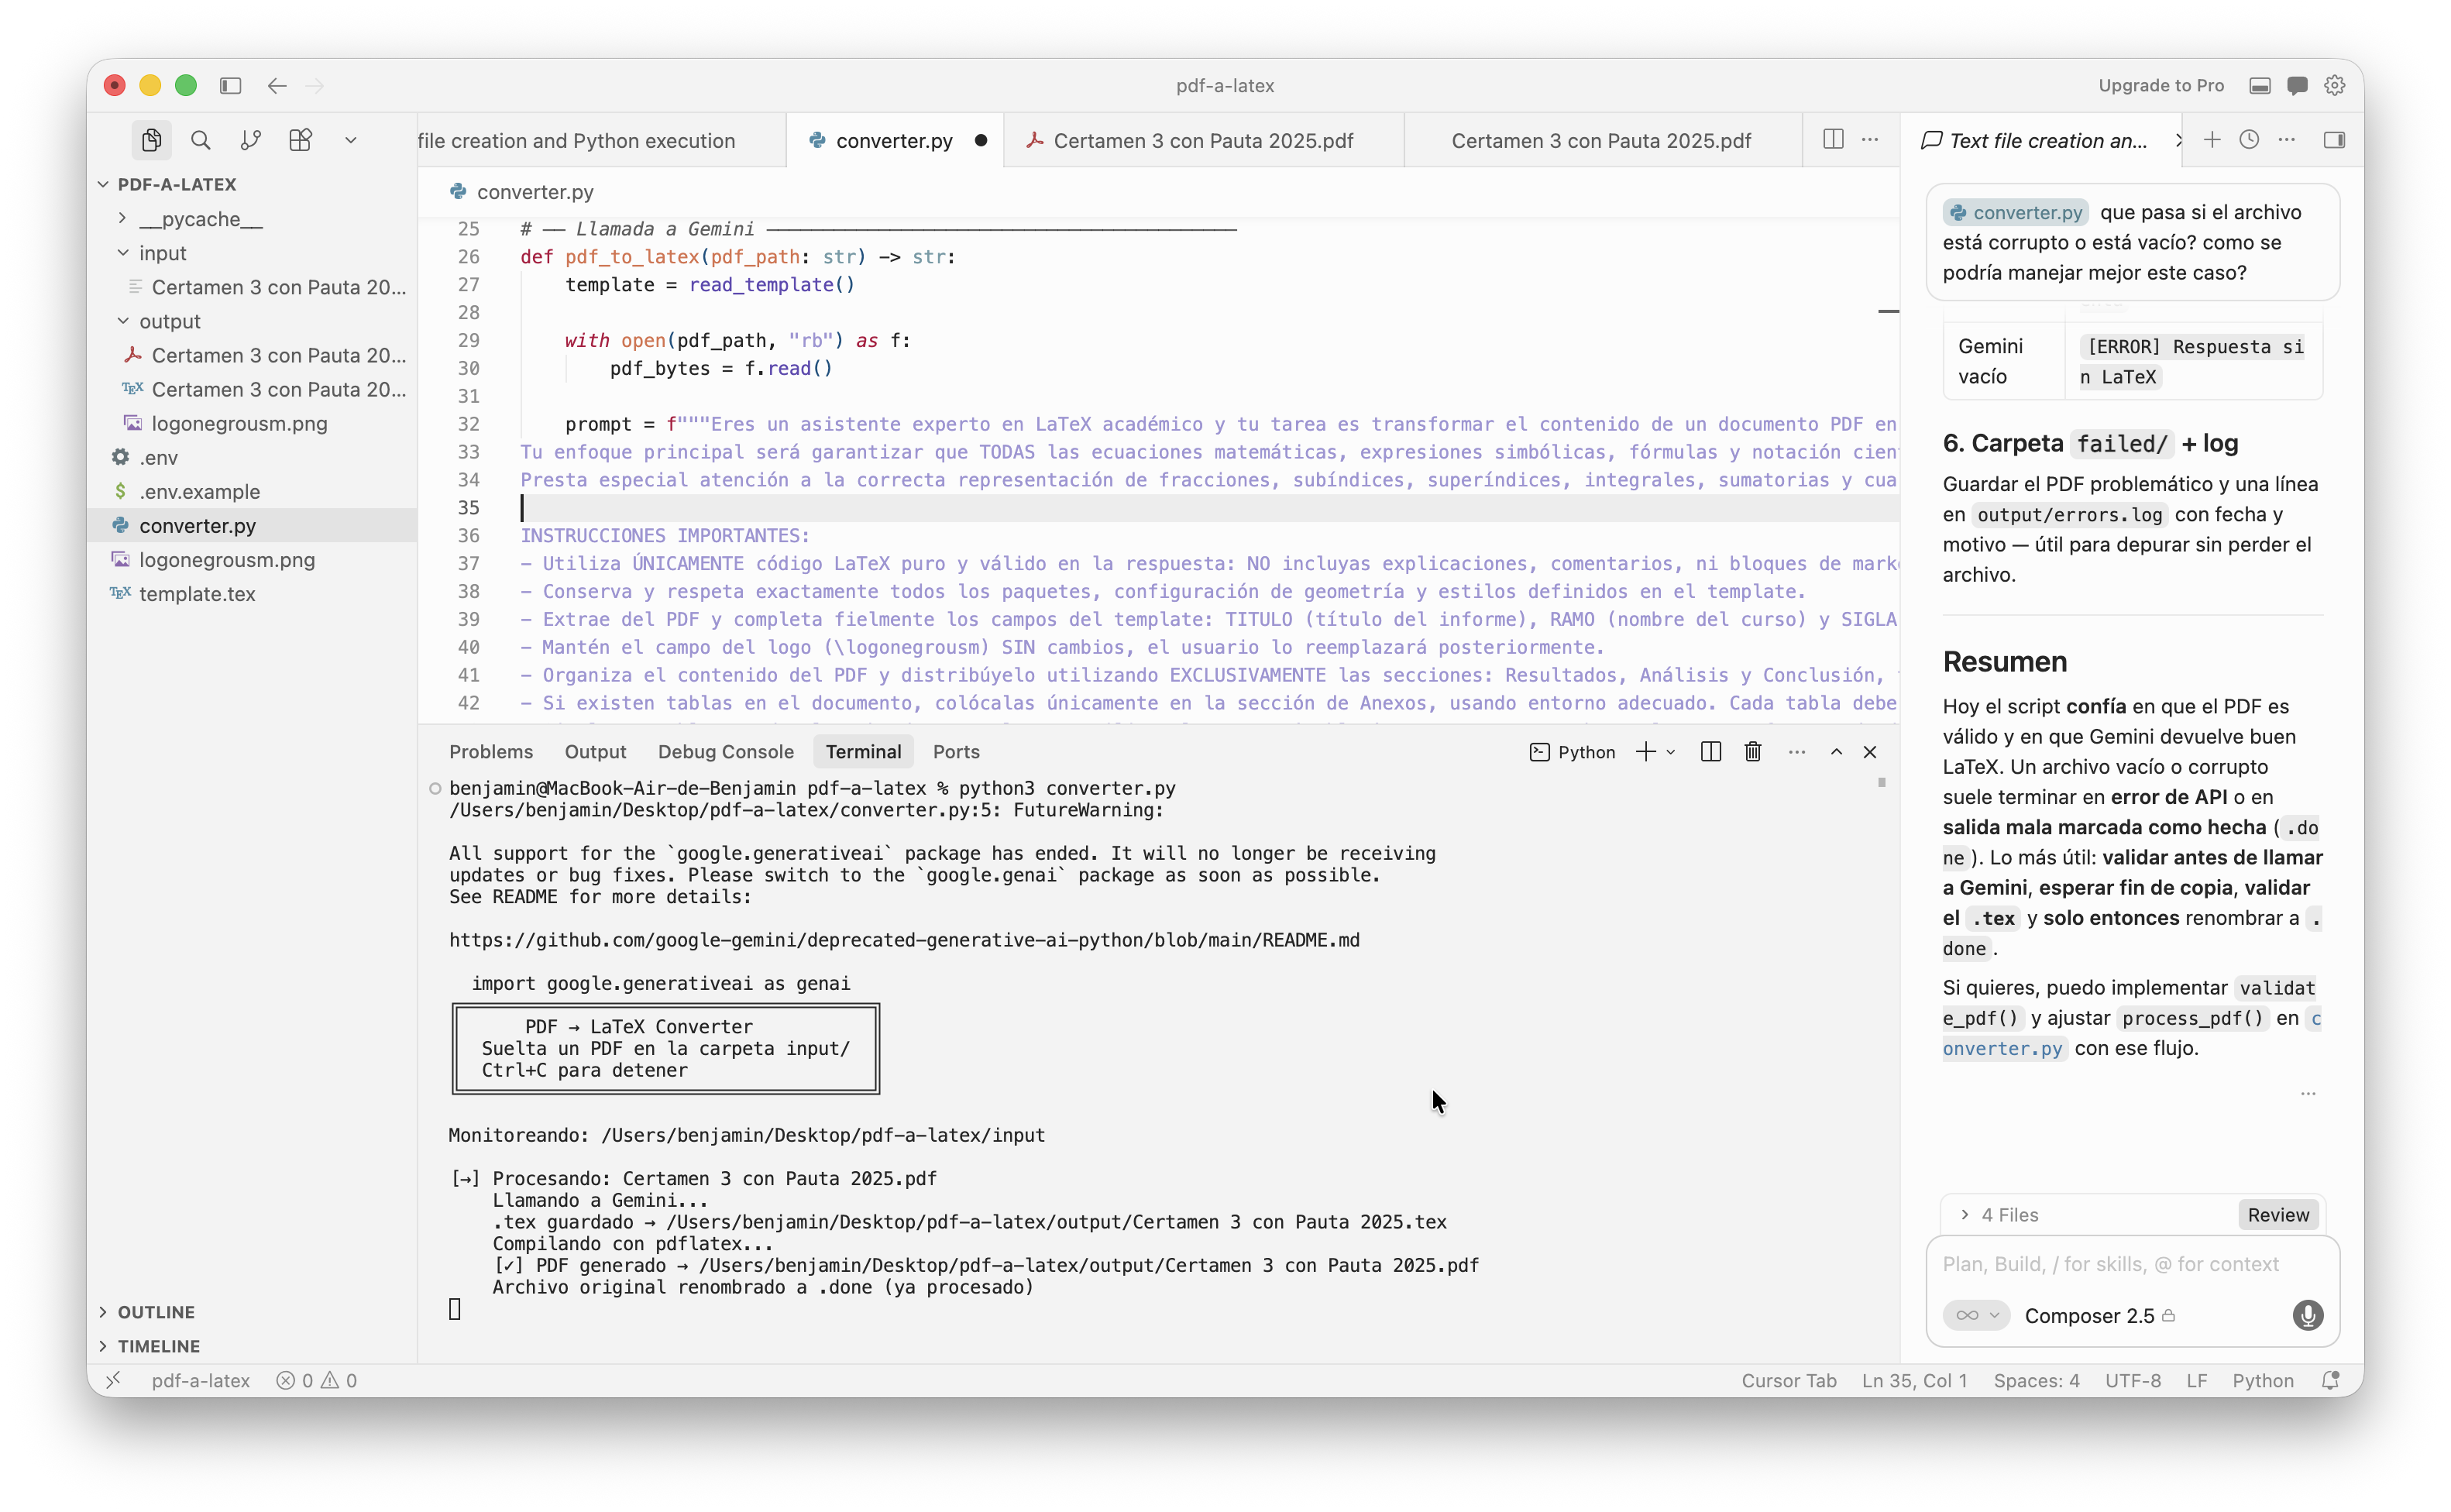
\includegraphics[width=0.5\linewidth]{Evidenciadeuso.png}
    \caption{Enter Caption}
    \label{fig:placeholder}
\end{figure}
\begin{figure}
    \centering
    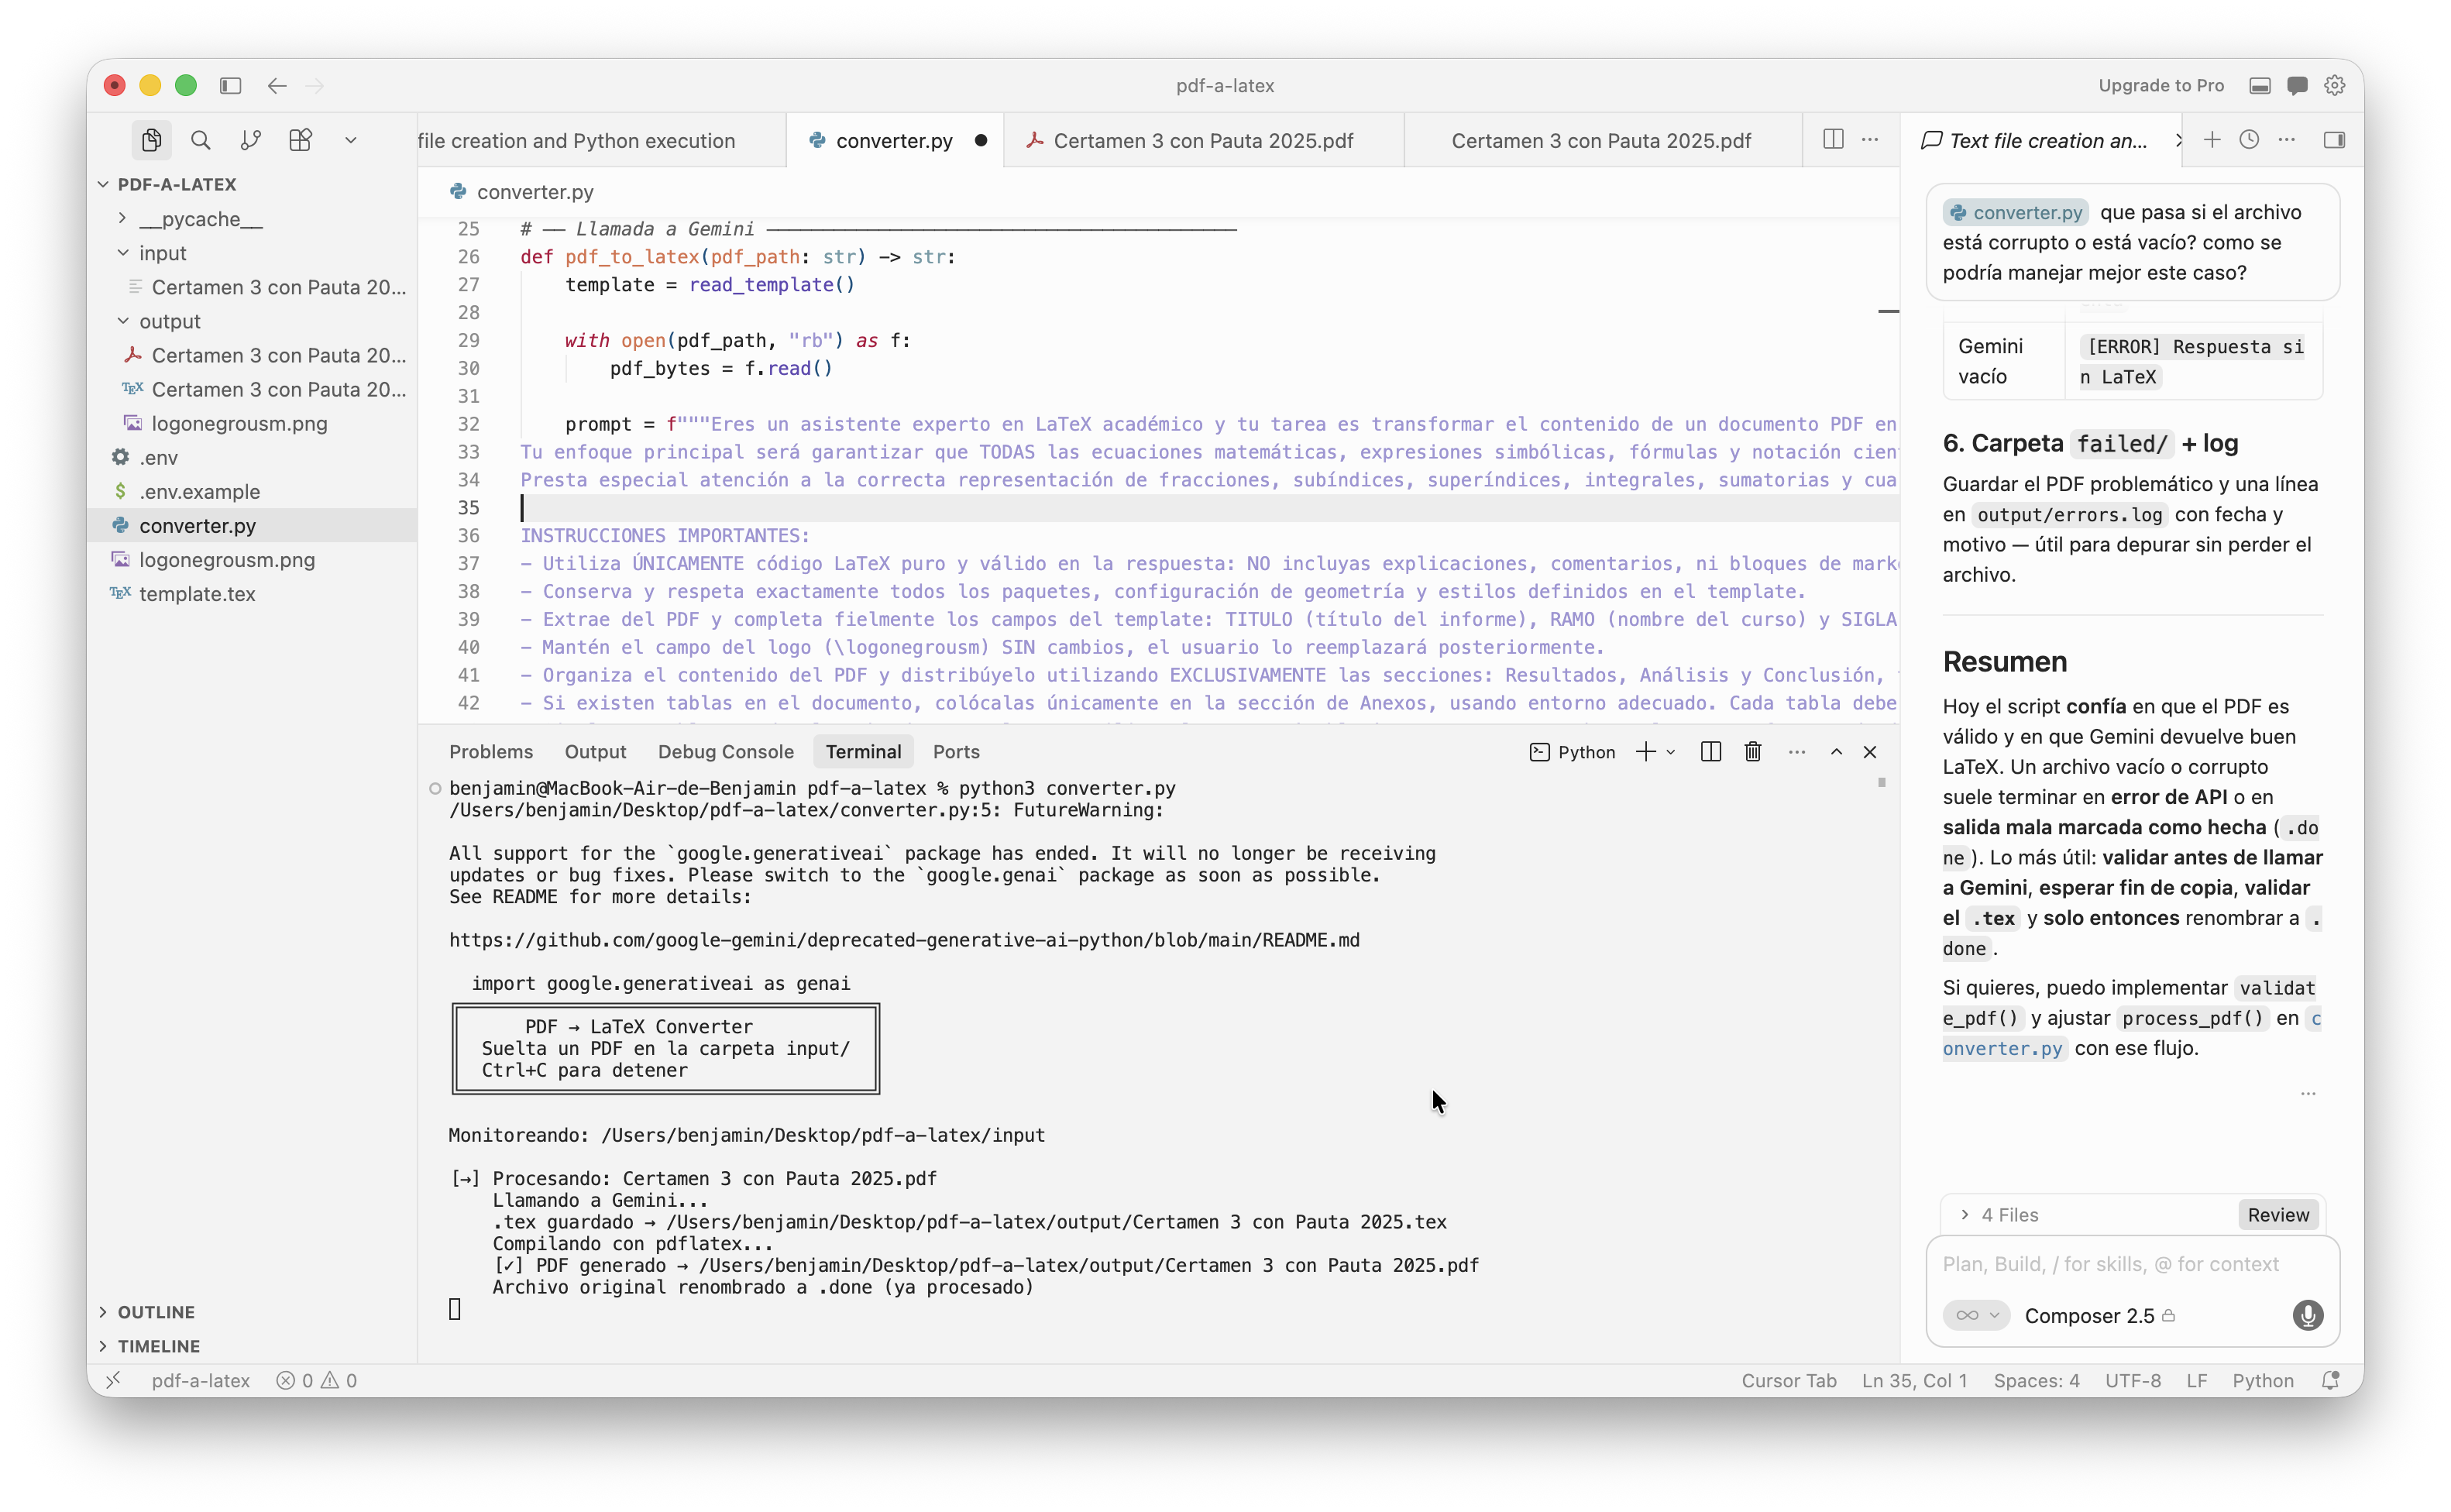
\includegraphics[width=0.5\linewidth]{Evidenciadeuso.png}
    \caption{Enter Caption}
    \label{fig:placeholder}
\end{figure}